\chapter{Conclusion and Future work}\label{chapter:conclusion_matter_evol}

\chapterabstract{In this chapter, I first conclude this part of the thesis, and outline several compelling questions and future applications arising from this work. Specifically, we discuss (1) whether the imaginary time period should be considered as an other additional boundary constraint, (2) whether the constraints derived in our model can be leveraged to theoretically predict cosmological parameters via thermodynamics, and (3) whether this framework could be used to indirectly detect non-trivial spatial topologies of the universe. Finally, we discuss the issue of negative matter density--as an odd function of scale factor, it switch signs when transitioning into the anti-universe. To resolve this paradox, we abandon the classical fluid approximation—which inevitably breaks down near cosmological singularities—and instead solve the fundamental quantum field equations near the Big Bang and the end of the universe. We validated this framework in scalar fields, and extending it to fermions naturally leads to the second part of the thesis.} 


\section{Conclusion}
In this Part of the thesis, we investigated the evolution of cosmological perturbations within a globally periodic universe. We derived analytic solutions to the first-order perturbation equations and imposed temporal boundary conditions (BCs) at the future conformal boundary (FCB). These conditions require the perturbations to be strictly symmetric or antisymmetric at the FCB, yielding a discrete spectrum of temporally allowed wave vectors. In \cref{chapter:theory}, we demonstrated that this temporally discrete spectrum is generically incompatible with the integer wave vectors demanded by the spatial compactness of a closed universe. However, because both sets of discrete \(k\) values exhibit equal, uniform spacing in the high-\(k\) regime, they can be formally reconciled by requiring the asymptotic spacing of the temporal modes to be an integer. Because this mode spacing is inversely proportional to the conformal age of the universe—a quantity highly dependent on spatial curvature—this matching condition rigidly constrains $\Omega_K$ to a specific set of discrete values. 

To facilitate a direct comparison with observational data, in \cref{chapter:Observation}, we evaluated the temporally discrete \(k\) spectrum by numerically solving the coupled perturbation equations, explicitly incorporating both matter and radiation anisotropies. The integer-spacing requirement was then utilized as a physical constraint to filter the \texttt{Planck 2018 MCMC} chains. This analysis yielded tight, predictive constraints not only on spatial curvature, but also on the broader set of background cosmological parameters that dictate the age of the universe. 

Finally, in \cref{chapter:low-k}, we extended this framework to the low-\(k\) regime, where the equal-spacing approximation fundamentally breaks down. We established that general solutions capable of satisfying both spatial and temporal BCs simultaneously must be constructed as linear combinations of the two respective bases. Geometrically, these physically valid solutions lie exactly at the intersection of the two basis subspaces, ensuring they remain invariant when projected back and forth between the spatial and temporal coordinate frames. Because the functional discrepancy between the two bases is highly significant at low frequencies, enforcing these dual constraints actively induces mode mixing and mode omissions. We subsequently generated the corresponding primordial and CMB power spectra from these unified solutions, revealing that the low-\(k\) modes exhibit a distinct power suppression accompanied by oscillatory features. Intriguingly, these theoretically derived signatures are phenomenologically consistent with long-standing anomalies observed in the CMB power spectrum.

\section{Future work}

In this section, we discuss three questions and future applications arising from this work. 

\subsection{Imaginary time period as an additional constraint}
Because the scale factor is periodic in both real and imaginary conformal time, one might ask whether the imaginary period imposes an additional boundary constraint on this model. The answer is no; only the real period dictates the physical boundary conditions for the perturbations. 

Consider a mode evolving as $\Phi\propto e^{i\omega t}$: it oscillates cleanly in real time but diverges exponentially in imaginary time. In standard calculations of gravitational entropy, integrating over the imaginary time period is mathematically valid because one first performs a Wick rotation, transforming the path integral $e^{iS}$ into an exponentially suppressed, well-behaved integral $e^{-S_E}$. However, when analyzing the dynamical evolution of physical perturbations in real spacetime (Lorentzian signature), only the real conformal time period imposes physical boundary constraints.

\subsection{Theoretical prediction of cosmological parameters}
Another compelling question is whether we can theoretically predict the values of other cosmological parameters using thermodynamic principles, bounded by the strict matching constraints derived in our model. This question is particularly interesting because Boyle and Turok \cite{2024PhLB..84938442B} demonstrated that universes with a smaller cosmological constant $\lambda$ and spatial curvature $\kappa$ possess higher gravitational entropy, making them statistically more probable. However, their framework could not predict the exact physical values of these parameters. 

To proceed, one could hypothetically calculate the thermodynamic expectation values of these parameters (where $S$ is the gravitational entropy). Taking the cosmological constant $\lambda$ as an example, the expectation value would be: 
\[ \big<\lambda\big>=\frac{\sum_{\lambda,r,m,\kappa}\lambda e^{S[\lambda,r,m,\kappa]}}{Z},\qquad Z=\sum_{\lambda,r,m,\kappa} e^{S[\lambda,r,m,\kappa]} \]

However, a critical problem arises: the partition function sum over the continuous parameter space diverges (e.g., as $\kappa\rightarrow 0$, $S\rightarrow\infty$). At first glance, our framework suggests a resolution, as it restricts the permissible cosmological parameters to a strictly discrete set. While this discretization might mathematically regularize the sum, the presence of an infinite sequence of discrete values approaching zero means the sum could still diverge under these constraints.

Alternatively, expectation values could be rigorously defined by differentiating the partition function, analogous to standard statistical mechanics: 
\begin{equation}
\begin{aligned}
    \big<E\big>&=\frac{\sum_E Ee^{-\beta E}}{Z},\qquad Z=\sum_E e^{-\beta E}\\
\rightarrow \big<E\big>&=-\partial_{\beta}\log Z
\end{aligned}
\end{equation}
Even if the raw partition function diverges, its logarithmic derivatives (and thus the physical expectation values) might remain finite and theoretically predictive.

\subsection{Detecting the topology of the universe}

While the most recent cosmological data are highly consistent with the simplest model of a zero-curvature, infinite universe, they remain equally compatible with compact topologies of homogeneous and isotropic geometries with small curvature. Examples include the spherical Poincaré dodecahedral space, the flat hypertorus, or the hyperbolic Picard horn.

There is no fundamental reason forcing space to possess a trivial topology. General relativity is a purely local theory; the Einstein field equations are local partial differential equations relating the metric and its derivatives to the matter-energy content at a specific point. Consequently, a single local metric solution to the Einstein equations can map to multiple—if not infinitely many—globally compatible topologies. For example, a compact hypertorus ($T^3$) and the standard infinite Euclidean space ($E^3$) are locally identical, and relativistic cosmological models describe them using the exact same FLRW equations. The only distinction lies in the global boundary conditions imposed on the spatial coordinates.

Is it possible to detect the global topology of the universe observationally? The search for such compact topologies, such as the hypertorus, is often termed \textit{cosmic crystallography}. Because the universe would be compact, an observer looking far enough would theoretically see repeating patterns or multiple images of the same structures. Observational efforts have attempted to identify such repeating patterns in large-scale structure distributions or within the cosmic microwave background (CMB). However, no conclusive evidence has been found. This null result implies either that the universe lacks a non-trivial global topology, or simply that the fundamental domain is significantly larger than our currently observable horizon. To learn more about the topology of the universe and how to observe it, one can refer to Jeffrey Weeks' book \textit{The Shape of Space} \cite{weeks2020shape}, which provides an excellent introduction to the topic.

Because it is difficult to observe the global topology directly if the fundamental domain is excessively large, one might ask whether it leaves an indirect signature that we can measure. Our framework offers a potential observational pathway. Different compact topologies impose varying spatial boundary conditions; our findings explicitly demonstrate that these conditions strictly quantize the allowed wave vectors. Consequently, the consistency requirement between the spatial and temporal boundary conditions imposes direct constraints on permissible universe topologies. For instance, if the universe is a hypertorus composed of periodic spatial 3D boxes, the physical dimensions of these boxes would rigidly dictate the minimum value and the exact spacing of the discrete wave vectors. Thus, the boundary matching evaluated in this work could serve as a novel method for indirectly probing the global shape of the universe.


\section{Matter field evolution near the Big Bang and the end of the universe}\label{sec:matter_evol} 

At the end of this part, we discuss the issue of negative matter density, which arise since the matter density is an odd function of scale factor $\Omega_m\paroto 1/a^3$, which switch signs when transitioning into the anti-universe. To resolve this problem, we states that near the transition point, i.e. the Bang and the end of the universe, the classical fluid approximation breaks down and the fundamental quantum field needs to be considered. And since the energy density is defined as absolute value of the field, it remains strictly positive. We demonstrate that scalar field solutions to the Klein-Gordon equation are natively symmetric at the Big Bang, whereas only massless scalar fields preserve this symmetry near the future conformal boundary. Finally, we discuss the extension of this framework to fermions, establishing the theoretical foundation for the investigations presented in Part II of this thesis.

\subsection{Negative matter density} 

Throughout this thesis, we evaluate solutions to the Friedmann equation within a periodic universe. However, a hidden theoretical problem arises regarding the matter density: 
\[ 3\frac{\dot a^2}{a^4}=\lambda +\frac{3\kappa}{a^2}+\frac{m}{a^3}+\frac{r}{a^4}, \]
where the terms proportional to $\lambda,\kappa,m,r$ correspond to the cosmological constant, spatial curvature, matter density, and radiation energy density, respectively. Note that the matter density term is the only strictly odd function of the scale factor $a$. This is not a problem when considering only our forward-evolving universe, where the scale factor $a$ remains strictly positive. However, when global periodic solutions are considered, the scale factor smoothly switches signs in the anti-universe (i.e., on the far side of the Big Bang and the Future Conformal Boundary). Naively, this causes the matter density to become negative. Because a strictly negative energy density is physically pathological, and because switching only the matter sign would cause an asymmetry in the global energy densities between the universe and the anti-universe, the symmetric evolution of $a(\eta)$ would be explicitly broken (see Sec.~V in \cite{2022PhRvD.105h3514L}). To resolve this problem computationally, we previously assumed that the matter density must always remain positive, scaling as $\rho_m\propto 1/|a|^3$. The primary goal of this chapter is to provide a rigorous theoretical justification for this absolute value assumption.

One natural hypothesis is that the relation $\rho_m\propto 1/a^3$ is strictly a classical approximation. This approximation is valid only when $H\ll \mu$ (i.e., far away from the initial singularity, when the ambient temperature is much lower than the fundamental particle mass $\mu$), where the matter smoothly behaves as a pressureless perfect fluid. However, when $H\gg \mu$ (i.e., infinitesimally close to the Big Bang), this fluid limit fails, and we must evaluate the evolution of the underlying quantum fields directly.

Specifically, in the regime where $1/H \sim t \gg 1/\mu$, sufficient time elapses for the high-frequency modes of the quantum field to complete numerous oscillations. These rapid oscillations average out, effectively validating the perfect fluid approximation where $\langle \sin(\mu t + kx) \rangle_{\text{oscillations}} \approx \text{fluid}$. In this limit, massive matter reliably behaves as a classical perfect fluid. On the other hand, in the opposite limit close to the Big Bang, where $1/H \sim t \ll 1/\mu$, the field did not have enough time to oscillate, so quantum effects become significant. 

Similarly, at the end of the universe (approaching the future de Sitter boundary, or FCB), the expansion rate $H$ begins to overwhelm the particle mass scale \footnote{Since particles become effectively massless at late times in de Sitter space, which we will discuss in the next section.}. When the exponential expansion of the de Sitter spacetime outpaces the quantum oscillations ($1/H \sim t \ll 1/\mu$), the field ceases to oscillate efficiently. Once again, the field dynamics cannot be time-averaged, causing the classical perfect fluid approximation to break down.

We propose the following theoretical mechanism: if one evaluates the exact quantum field equations near the Big Bang and the FCB, the fundamental energy density of the fields remains strictly positive. For a canonical scalar field, the energy density evaluates to $\rho \propto \frac{1}{2}(\mu^2 + k^2)\phi^2 > 0$. Therefore, when the classical fluid approximation is recovered at intermediate times (far from the singularities), it naturally enforces the effective scaling $\rho_m\propto 1/|a|^3$.

\subsection{Toy model: The scalar field}

To rigorously test this hypothesis, we first analyze the simplest available model: a free scalar field governed by the Klein-Gordon equation. 

The equation of motion for a scalar field in an expanding universe is $\ddot{\phi} + 3H\dot{\phi} + (k^2/a^2 + \mu^2)\phi = 0$, where the dots denote derivatives with respect to physical time $t$. Transforming this equation into conformal time ($\eta$) yields: 
\[ \ddot{\phi} + 3\frac{\dot{a}}{a}\dot{\phi} + (k^2 + \mu^2a^2)\phi = 0, \quad \text{(where dots now denote } d/d\eta \text{)}. \]

To investigate its geometric evolution near the Big Bang, we apply the radiation-dominated limit, $a \propto \eta$. The analytic solutions can be expressed in terms of the confluent hypergeometric function $U$ and the generalized Laguerre polynomial $L$:

\begin{equation}\label{eq:scalarfield_sol_BB}
    \phi_1(\eta )= \frac{ e^{\frac{1}{2} i \mu\eta ^2 } U\left(-\frac{i k^2}{4 \mu},0,-i \mu \eta ^2\right)}{\eta ^2},\qquad
    \phi_2(\eta)=\frac{ e^{\frac{1}{2} i \mu\eta ^2 } L\left({\frac{i k^2}{4 \mu}},-1,-i \mu \eta ^2\right)}{\eta ^2}.
\end{equation}

\cref{fig:scalarField_sol_BB} plots the absolute value of these two independent solutions ($|\phi_1|$ and $|\phi_2|$) in blue and orange, respectively, with $k=\mu=1$. The second solution, $|\phi_2|$, is the physically valid mode because it remains finite exactly at the Big Bang singularity. Crucially, this physical solution is perfectly symmetric before and after the Bang, robustly confirming the global periodic universe paradigm and inherently preserving a positive-definite energy density.

\begin{figure}
     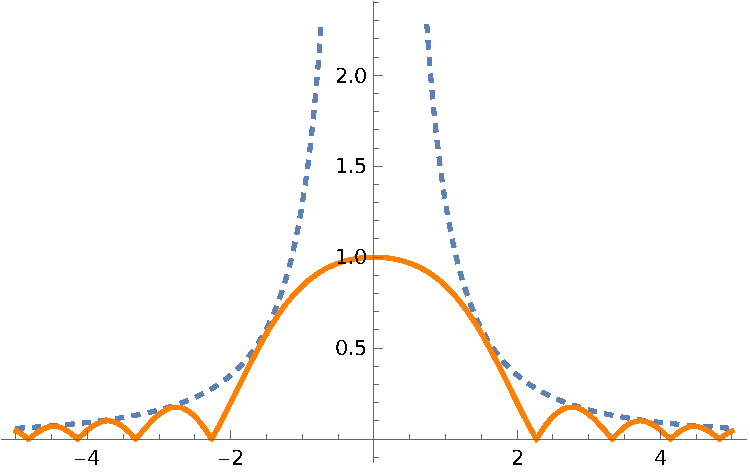
\includegraphics[width=0.5\textwidth]{figures/scalarField_sol_BB.pdf}
     \centering
     \caption{Absolute value of the scalar field solutions near the Big Bang ($\eta=0$). We plot $|\phi|$ because physical energy density is governed by the field amplitude squared.}
     \label{fig:scalarField_sol_BB}
\end{figure}

Next, we evaluate the field evolution near the future conformal boundary (FCB). Modeling the asymptotic de Sitter approach as $a \propto 1/\sqrt{\lambda}(\eta_\infty-\eta)$, the analytic solutions take the form of Bessel functions ($J$ and $Y$): 

\begin{equation}\label{eq:scalarfield_sol_FCB}
    \phi_1(\eta )= \frac{ J_{\sqrt{\frac{\lambda -\mu^2}{\lambda }}}(k \eta -k \eta_{\infty})}{\eta_{\infty}-\eta },\qquad 
\phi_2(\eta)=\frac{ Y_{\sqrt{\frac{\lambda -\mu^2}{\lambda }}}(k \eta -k \eta_{\infty})}{\eta_{\infty}-\eta }.
\end{equation}

\cref{fig:scalarField_m=1_sol_FCB} plots the absolute amplitudes of these solutions (with parameters set to $k=1, \mu=1, \lambda=1,$ and $\eta_\infty=0$). In the presence of a non-zero mass, both independent solutions diverge to infinity at the FCB, rendering them physically pathological.

\begin{figure}
     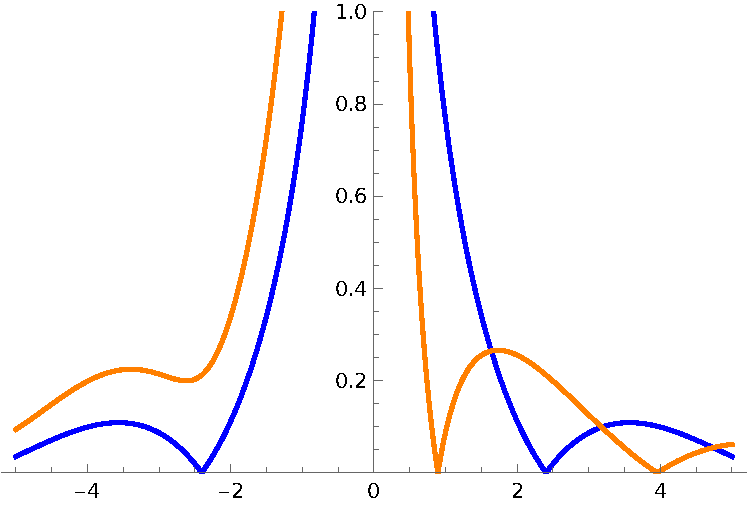
\includegraphics[width=0.5\textwidth]{figures/scalarField_m=1_sol_FCB.pdf}
     \centering
     \caption{Absolute value of the massive scalar field solutions ($|\phi|$) approaching the future conformal boundary ($\eta_\infty=0$). Both solutions are physically divergent.}
     \label{fig:scalarField_m=1_sol_FCB}
\end{figure}

However, if we take the strict massless limit ($\mu\to 0$), the geometric pathology resolves. One of the solutions becomes finite and perfectly symmetric across the boundary:
\begin{figure}
     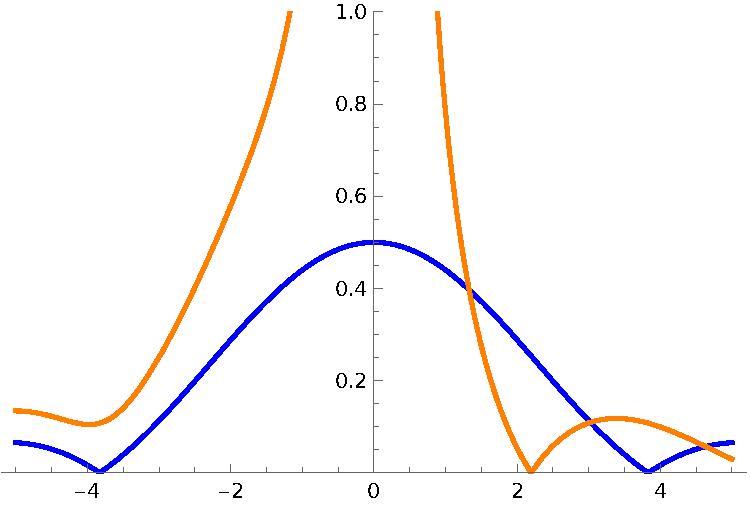
\includegraphics[width=0.5\textwidth]{figures/scalarField_massless_sol_FCB.pdf}
     \centering
     \caption{Absolute value of the nearly massless scalar field solution ($\mu=0.001$) near the end of the universe ($\eta_\infty=0$). The solution is finite and globally symmetric.}
     \label{fig:scalarField_massless_sol_FCB}
\end{figure}

This analysis reveals a profound theoretical constraint: if we couple a massive field ($\mu \neq 0$) to gravity in the standard manner, its quantum mode functions encounter an essential singularity at the future de Sitter boundary. Physically, this occurs because the field attempts to oscillate an infinite number of times (with frequency $\propto \mu$) as coordinate time stretches to infinity near the boundary. Consequently, a stable, well-behaved future boundary condition (such as an analytic Neumann or Dirichlet condition) cannot be imposed. 

However, if physical fields couple to gravity in a non-standard (e.g., strictly Weyl-invariant) fashion—such that their effective mass systematically vanishes as the universe approaches the FCB—well-defined future boundary conditions become theoretically permissible. Several physical mechanisms could drive this effectively massless limit. One possibility is universal particle decay (e.g., proton decay), wherein all massive states eventually decay into massless, strictly Weyl-invariant radiation prior to the FCB. Another highly compelling possibility relates to the ultimate fate of cosmic expansion (the "Big Rip" scenario): as the universe expands exponentially, all bound structures, and eventually the fundamental particles themselves, are torn apart. Once a particle's Compton wavelength is stretched beyond the radius of the observable causal horizon, the particle dynamically ceases to behave as a massive state, rendering the entire field effectively massless as it approaches the conformal boundary.

\subsection{The extension to fermions}

Because macroscopic matter is fundamentally composed of fermions rather than bosons, confirming this absolute-value energy scaling requires a rigorous evaluation of the Dirac equation. Several studies have attempted to solve the Dirac equation exactly within the FLRW metric. A foundational analysis by \citet{PhysRevD.36.3705} provided solutions for scale factors evolving as $a\propto t$, $a\propto t^{1/2}$, and $a\propto e^{Ht}$. This framework was later generalized to spatially curved universes by \citet{Huang:2005rn}. More recently, \citet{Ibison11} reformulated the field equations in conformal time, explicitly discussing their asymptotic behavior near the future conformal boundary.

However, treating spin-1/2 particles in these extreme limits is mathematically fraught. Near both the initial singularity and the future de Sitter boundary, the intensely curved spacetime violently mixes the internal spinor components via the dynamic spin connection, rendering certain components fundamentally unphysical \cite{Ibison11}. 

Is there a mathematically more elegant way to evaluate the boundary evolution of fermions? This precise question motivates the second half of this thesis, which deeply investigates the properties of Kähler-Dirac (KD) fermions. Because KD fermions are mathematically formulated using differential exterior forms (traditionally representing bosonic fields), we can initially solve the well-behaved field equations for bosons, and subsequently use those geometric solutions to rigorously reconstruct the exact fermionic dynamics. This indirect technique is potentially far more robust than attempting to solve the highly coupled, spin-connected Dirac equation directly. Before executing this methodology, however, we must systematically map the fundamental physical properties of KD fermions and establish their broader implications for both cosmology and the Standard Model.


\printbibliography[heading=subbibintoc, title={References for Chapter \thechapter}]
